\section[MODELO DE ARQUITETURA]{MODELO DE ARQUITETURA}

O modelo de arquitetura no seu nível mais elevado, pode ser visto como um modelo de três camadas, conforme a Figura \ref{camadas_arquitetura}.
\begin{figure}[ht]
	\centering
	\includegraphics[width=7cm]{figuras/camadas.eps}
	\caption{Camadas arquiteturais.}
	\label{camadas_arquitetura}
\end{figure}

A camada \emph{web} é responsável pela interação com o usuário. 
A camada \emph{Web API} é responsável pela lógica de negócio. 
A camada de base de documentos é responsável pela persistência dos dados da aplicação.


\subsection[CAMADA DE APLICAÇÃO WEB] {CAMADA DE APLICAÇÃO WEB}
Esta camada foi projetada para rodar em \emph{browsers} que suportam \emph{HTML} 5. 
Ela é desenvolvida usando-se \emph{Javascript}, \emph{CSS} e \emph{HTML}. 
Além disso, adotou-se o \emph{framework} de desenvolvimento \emph{web} \emph{AngularJS}, ver \ref{angularjs}. 

Como o projeto não possuía recursos adequados a criação de uma equipe de desenvolvimento \emph{web} completa, afim de se minimizar os problemas com \emph{design web}, optou-se por usar a biblioteca \emph{angular-material}, ver \ref{angular_material}. 

A Figura \ref{material_amostra}, mostra um exemplo de uma tela criada com as diretivas do angular-material. Note que todo o \emph{look and feel} da tela é determinado pelo comportamento padrão da biblioteca.

\begin{figure}[ht]
	\centering
	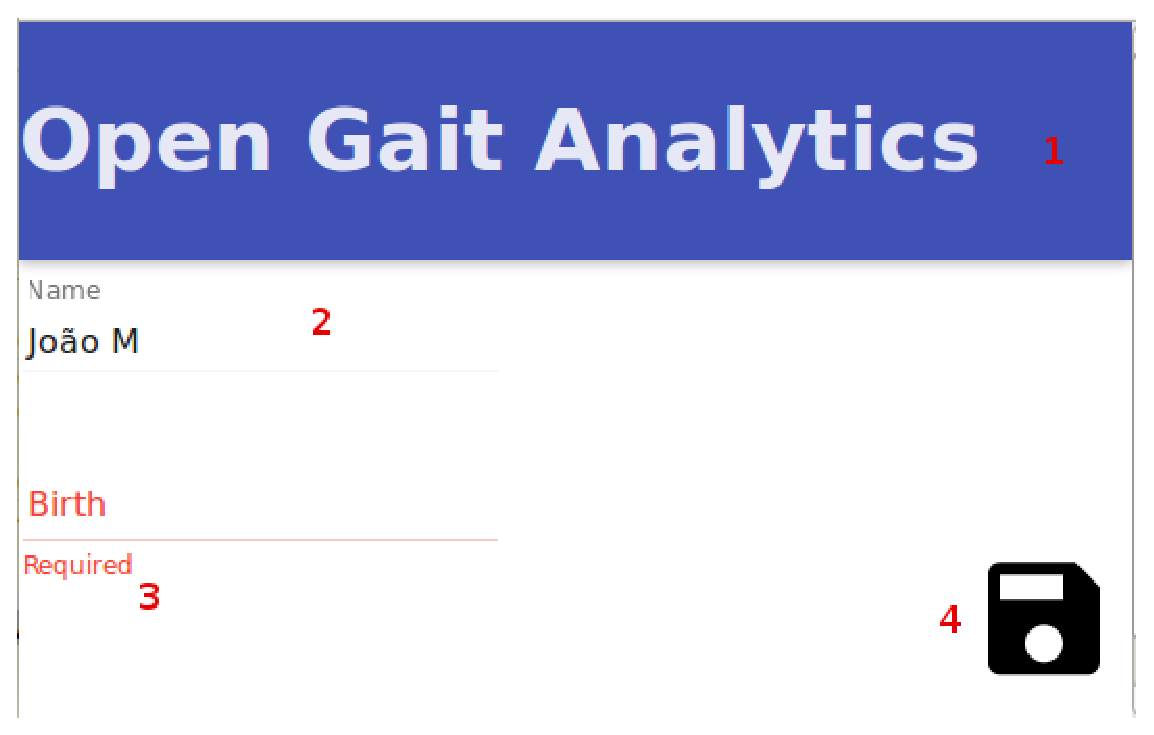
\includegraphics[width=9cm]{figuras/material_amostra.eps}
	\caption[Exemplo de uma tela criada com \emph{angular-material}.]{Exemplo de uma tela criada com \emph{angular-material}. 1) Diretiva \emph{md-toolbar}}; 2) Diretiva \emph{md-input-container}; 3) Diretiva \emph{ng-messages} em conjunto com a \emph{md-input-container}; 4) Diretiva \emph{md-button}.
	\label{material_amostra}
\end{figure}

\textbf{ORGANIZAÇÃO DO CÓDIGO FONTE}

A criação de um ambiente de desenvolvimento \emph{web}, para um software de média para grande complexidade, não é uma tarefa trivial de ser resolvida.
É necessários criar padrões de organização de arquivos, configurar e instalar pacotes de software para desenvolvimento, testes, implantação, construção de \emph{builds}, entre outros.
Para facilitar esta tarefa, optou-se em utilizar o projeto \emph{angular-seed}, ver \ref{angular_seed}.
A ideia deste projeto é servir de esqueleto de projetos \emph{web} que utilizam o \emph{framework} \emph{AngularJS}.
Para usar este projeto basta cloná-lo diretamente do seu repositório \emph{git} no \emph{site} github.com, conforme o comando abaixo.
\lstset{language=bash}
\begin{lstlisting}[frame=single]
git clone https://github.com/angular/angular-seed.git
\end{lstlisting}

Antes de começar a usar o \emph{angular-seed} é necessário instalar o ambiente de execução \emph{Javascript Node.JS}. 
Este ambiente é utilizado para execução de testes e construção de \emph{builds}. Para uma introdução ao \emph{Node.JS} veja \citeonline{Syed2014}.
